\documentclass[runningheads,a4paper]{llncs}

\usepackage{amssymb}
\setcounter{tocdepth}{3}
\usepackage{graphicx}
\usepackage{tikz}
\usepackage[T1]{fontenc}
\usepackage[scaled]{beramono}
\usepackage{listings}
\usepackage{color}
\usetikzlibrary{arrows,chains,positioning,scopes,quotes,calc}

\newcommand{\keywords}[1]{\par\addvspace\baselineskip
\noindent\keywordname\endspace\ignorespaces#1}
\pagestyle{plain}
\setlength\parindent{0pt}

\definecolor{mygreen}{RGB}{28,172,0} % color values Red, Green, Blue
\definecolor{mylilas}{RGB}{170,55,241}

\newcommand*{\StrikeThruDistance}{0.15cm}%
\newcommand*{\StrikeThru}{\StrikeThruDistance,\StrikeThruDistance}%

\tikzset{strike thru arrow/.style={
    decoration={markings, mark=at position 0.5 with {
        \draw [blue, thick,-] 
            ++ (-\StrikeThruDistance,-\StrikeThruDistance) 
            -- ( \StrikeThruDistance, \StrikeThruDistance);}
    },
    postaction={decorate},
}}

\lstset{
  language=Python,
  showstringspaces=false,
  formfeed=\newpage,
  tabsize=4,
  commentstyle=\itshape,
  basicstyle=\ttfamily,
  morekeywords={models, lambda, forms}
}

\begin{document}
\def \SystemName {Worlds} % Lol because this shit probably will change.

\mainmatter  % start of an individual contribution

% This needs some work, big time.
\title{\SystemName: A distributed MMO \textit{(DRAFT)}}

\author{Ryan Walker\\
				ryan.cjw@gmail.com}

\institute{} %Merp

\maketitle
%% Serious scrum area
% Player Experience points
%		- How does this transcend worlds.
%		- This should be
% Zero Sum currency
% 	- Based on an existing crypto
%		- Has exchangeability for real monies
%		- Worlds are trying to generate this
%		- This can be done by
%			- Offering exchangeability for a token that world offers
%			- Charging an entrance fee
%			- Charging for items
% Game theoretical elements
%			- Worlds want players to play in their world
%			- They want to have
%				- Common item exchange between worlds
%				- Experience dished out to be recognised 

\begin{abstract}
A protocol defining how anyone can contribute to an unbounded universe could allow the flexibility to organically grow an MMO faster than any proprietary system. This paper overviews a protocol that enables developers to bolt their game into in common universe. 
\end{abstract}

\section{Introduction}
For an open software ecosystem to grow organically there should be outlets for contribution. In the context of a massively multiplayer online game the outlets become more complicated then a simple code repository. Fair game mechanics are built on a fragile ecosystem that have negative consequences if managed improperly. The fairness and security of a game are dependent on it's network forming consensus. This is trivially done with conventional methods. A server maintains a secure connection with a player who pipes actions to the server. The server then provides ground truth for the network. Distributed systems require a very different approach. Blockchains present clear deficiencies, they are too slow and the chain would get too large. An alternate method will now be presented.

\section{Worlds}
\subsection{Overview}
% A node the hosts players and provides an experience 
% Provides that game client that renders player graphics
% Hosts servers that run the worlds engine

A world, defined as $w_k$, is a node that designs a user experience and hosts players. Worlds provide the game client that players interact with. In addition they host servers that form consensus among the worlds domain. A world can have up to four adjacent worlds determined by itself. Players, defined as $P_k$, can enter a world one of three ways. The first being a \textbf{player genesis}(\ref{PG}). The second being a \textbf{world transfer} (\ref{WT}) and the third: a \textbf{refuge packages}(\ref{RP}). It is possible for players to transfer between adjacent worlds and keep their items and stats. This is done using the mechanics discussed below.

\begin{small}
\tikzset{myblock/.style = {rectangle, draw, minimum height=1cm, minimum width=3cm}}
\begin{center}
\begin{tikzpicture}
\label{Hello}
\node(WE)[myblock]{\begin{tabular}{c}Worlds Engine \\ {\scriptsize wClient.py} \\\end{tabular}};
\node (WS)[myblock,above of=WE, yshift=1cm]{\begin{tabular}{c}Worlds Server \\ {\scriptsize wServer.py} \\\end{tabular}};
\node (WC)[myblock,left of=WE, xshift=-3cm]{\begin{tabular}{c}Game Client \\ {\scriptsize \textit{From game Dev}} \\\end{tabular}};
\node (SE)[myblock,left of=WS, xshift=-3cm]{\begin{tabular}{c}Server Engine \\ {\scriptsize \textit{From game Dev}} \\\end{tabular}};

\draw [dashed] (-6,1) -- (6,1);
\node [right of=WS, xshift=2cm]{Server Side};
\node [right of=WE, xshift=2cm]{Client Side};

\draw[->] ($(WE.north east)!0.25!(WE.north west)$) --  ($(WS.south east)!0.25!(WS.south west)$);
\draw[<-] ($(WE.north east)!0.75!(WE.north west)$) --  ($(WS.south east)!0.75!(WS.south west)$);
\draw[->] (WC) -- (WE);
\draw[->] (SE) -- (WS);

% more arrows here
\end{tikzpicture}
\end{center}
\end{small}

\subsection{Action Ledger}
\label{AL}
An action ledger, defined as $AL(P_{k}, w_k)$, is a chronological list of all the signed actions and reactions that has happened to a player in a world. In order to commit an action a player must concatenate a nuance with the action, then sign and send to the world. If the action is legal, it is entered into the world's action ledger for that player. If reactions are to occur to a player, the world must follow the same process and send the signed payload to the players. Players are required to keep their actions ledger dating back to their genesis, worlds are only required to keep \textbf{transport hashes} (\ref{TH}).

\subsection{Transport Hash}
\label{TH}
A transport hash is a hash of an action ledger, $h_s(AL(P_{k}, w_k))$, these are secured by the worlds and are used to prove a player is presenting an honest action ledger. The transport hash is formed when a player leaves the world. A \textbf{Forward Transport Hash} is a transport hash kept in a special location. This is explained more in the world transfer section, it is defined as  $h_{sf}(AL(P_{k}, w_k))$.

\subsection{World Transfer} 
\label{WT}
A detailed state machine outlines how players can move about neighboring worlds. Honest worlds must follow this procedure, if they misbehave they could be risking a \textbf{World Disconnect} (\ref{WD}) from their neighboring worlds. 
\\
\\
\textbf{Eg:} A player, defined as $P_1$, wants to move from $w_1$ to $w_2$ and then to $w_3$ (Figure \ref{w1tow2}), The network values in this scenario are defined as...

\begin{figure}
\caption{$P_1$ moving from $w_1$ to $w_2$}
\label{w1tow2}
\begin{center}
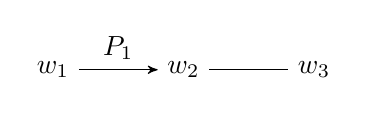
\begin{tikzpicture}[>=stealth']
{[start chain]
\node[on chain] (A) {$w_1$};
\node[on chain,join=by {->,"$P_1$"},right=of A] (B) {$w_2$};
\node[on chain,join=by {-},right=of B] (C) {$w_3$};}
\end{tikzpicture}
\end{center}
\begin{center}
\begin{tabular}{ c|c c c }
& $w_1$ & $w_2$ & $w_3$ \\
\hline 
$h_s(AL(P_1,w_k))$ & $NULL$ & $NULL$ & $NULL$ \\ 
$h_{sf}(AL(P_1,w_k))$ & $NULL$ & $NULL$ & $NULL$ \\ 
Neighbor & $w_2$ & $w_1$ \& $w_3$ & $w_2$\\
\end{tabular}
\end{center}
\end{figure}

\begin{enumerate}
\item $P_1$ sends a signed world entry packet to $w_2$
\item $w_2$ insures that $w_1$ is adjasent to itself
\item $w_2$ must verify that $P_1$ currently resides in $w_1$, this is done by ensuring $h_{sf}(AL(P_1,w_k)) = NULL$. This is found by sending a signed data request to $w_1$ 
\item $P_1$ presents $AL(P_1,w_1)$ to $w_2$
\item $w_1$ calculates $h_s(AL(P_1,w_1))$ using the $AL$ on the serverside
\item $w_2$ calculates $h_s(AL(P_1,w_1))$ using the $AL$ provided by $P_1$, the hashes must match
\item (Optional) An \textbf{Action Ledger Traceback} (\ref{ALT}) can be complete
\item $P_1$ is now granted access to $w_2$ and can submit actions
\item $w_1$ must store $h_s(AL(P_1,w_1))$, $AL(P_1,w_1)$ can be deleted
\end{enumerate}

\begin{figure}
\caption{$P_1$ in $w_2$}
\begin{center}
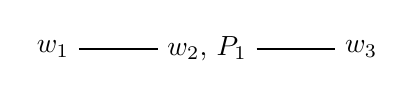
\begin{tikzpicture}[>=stealth']
{[start chain]
\node[on chain] (A) {$w_1$};
\node[on chain,join=by {-},right=of A] (B) {$w_2$, $P_1$};
\node[on chain,join=by {-},right=of B] (C) {$w_3$};}
\end{tikzpicture}
\end{center}
\begin{center}
\begin{tabular}{ c|c c c }
& $w_1$ & $w_2$ & $w_3$ \\
\hline 
$h_s(AL(P_1,w_k))$ & $ h_s(AL(P_1,w_1))$ & $NULL$ & $NULL$ \\ 
$h_{sf}(AL(P_1,w_k))$ & $NULL$ & $NULL$ & $NULL$ \\ 
Neighbor & $w_2$ & $w_1$ \& $w_3$ & $w_2$\\
\end{tabular}
\end{center}
\end{figure}

\begin{figure}
\caption{$P_1$ in $w_3$}
\begin{center}
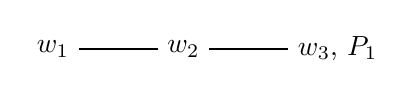
\begin{tikzpicture}[>=stealth']
{[start chain]
\node[on chain] (A) {$w_1$};
\node[on chain,join=by {-},right=of A] (B) {$w_2$};
\node[on chain,join=by {-},right=of B] (C) {$w_3$, $P_1$};}
\end{tikzpicture}
\end{center}
\begin{center}
\begin{tabular}{ c|c c c }
& $w_1$ & $w_2$ & $w_3$ \\
\hline 
$h_s(AL(P_1,w_k))$ & $h_s(AL(P_1,w_1))$ & $h_s(AL(P_1,w_2))$ & $NULL$ \\ 
$h_{sf}(AL(P_1,w_k))$ & $h_s(AL(P_1,w_2))$ & $NULL$ & $NULL$ \\ 
Neighbor & $w_2$ & $w_1$ \& $w_3$ & $w_2$\\
\end{tabular}
\end{center}
\end{figure}

\subsection{Player Genesis} 
\label{PG}
Player Genesis is the creation of a new player, for this to occur a player must digitally sign a genesis package with unix time. The world must ensure there are no existing values entered for that player. The player is then instated into the world with all the initial player values set to zero. 

\subsection{Refuge Package}
\label{RP}
A refugee package is an action ledger that dates to the time that the package is sent. This allows worlds to reinstate players without the need of a world transfer. This is useful for player that have been orphaned into a world. This typically happens during either a \textbf{world disconnect} (\ref{WD}) or \textbf{world outage} (\ref{WO}). This has the effect of splitting the player's history into two forks, which opens the possibility of an \textbf{action ledger conflicts} (\ref{ALC}).

\section{Engine Mechanics} 
The mechanics below are simply suggestions. As the engine is completely open, worlds are free to impose whatever mechanics they wish. Worlds with drastically different game mechanics will probably not be bordering, this limits gameplay but maintains fairness. Players are able to play in whatever worlds they wish - but they must start from scratch in non-adjacent clusters.

% Clusters of worlds might be complete anarchy, others built on peace and justice. There will probably not be a connection between sections like this, which is perfectly fine.

\subsection{Action Ledger traceback}
\label{ALT}
The system is not entirely trustless, the neighboring worlds need to trust each other. It is possible for neighboring worlds to have disagreements and still function. For instance, $w_1$ might introduce an item that $w_2$ considers too powerful. In a case like this $w_1$ world can just neglect it. Actions presented using that item would be considered illegal and not entered into the action ledger of the $w_1$. Worlds that are not entirely trusted can be audited, consider Figure \ref{ThreeW} 

\begin{figure}
\caption{Three adjacent worlds}
\label{ThreeW}
\begin{center}
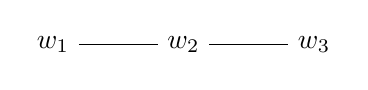
\begin{tikzpicture}[>=stealth']
{[start chain]
\node[on chain] (A) {$w_1$};
\node[on chain,join=by {-},right=of A] (B) {$w_2$};
\node[on chain,join=by {-},right=of B] (C) {$w_3$};}
\end{tikzpicture}
\end{center}
\end{figure}

It is possible that $w_1$ might have conflicts with the rules of $w_3$, however $w_1$ did not choose be adjacent to $w_2$. During the worlds transfer, $w_1$ would not get the action ledger from $w_3$. Completely illegal action could have been committed in $w_3$ (eg. free money). In this case $w_1$ can request an \textbf{Action Ledger Traceback}(\ref{ALT}). If this is requested, the player must provide a list of action ledgers that date back to either the player genesis or to the last entry of the world committing the audit. The world then needs to obtain $h_s{AL(P_k, w_{k:n})}$ from $w_k$ to $w_n$. If the hashes match then the players history has been confirmed. 
\\\\
Below are some mechanics that can be employed to combat illegal actions.

% If $AL(P_k, w_{k:n})$ contains illegal actions, 

% there are three ways of dealing with this. The first is to issues a disconnect from $w_2$, this has the disadvantage of players now not being able to travel to $w_2$. The second is to change the rules. The third way to is implement a one-way-gate. This is a method of ensuring that illegal rules don't make their way into the issuing world.

\subsection{World Disconnects}
\label{WD}
It is possible a world may issue a disconnect of an adjacent world, this means that players may no longer travel between these worlds. This is considered to be the more drastic and can leave players orphaned in the disconnected world, see \textbf{Orphaned Players} (\ref{OP}).

% It would be logical for the world that issued the disconnect to accept \textbf{refugee packages} (\ref{RP}) from the orphaned player. The history of that player is now forked into two separate paths as the player will still be able to play on either worlds. It would be highly risky for the player to play on both accounts as it could risk an \textbf{action ledger conflict}(\ref{ALC})


% \node (WS)[myblock,above of=WE, yshift=1cm]{Worlds Server};

\subsection{One Way Gates} % This needs rework.
Worlds can only control their adjacent neighbors, they have no way of controlling the neighbors of their neighbors. Consider Figure \ref{ThreeW} If $w_1$ issues a one-way-gate against $w_3$ player are no longer allowed to travel back into $w_1$ if they have traveled through $w_3$.

\subsection{World Economic Caps}
It's possible that worlds may require neighboring worlds to employ a \textit{world economic cap}. This sets a hard cap to the amount of resources that can be distributed to players from the environment in a given time period. This can cap experience points, coins, items, etc...

\subsection{Item Ledger}
\label{shIL}
Worlds with greater security requirements might require an item ledger upon world transfers. An item ledger is a data construct the holds an item's history. The first entry should be the items genesis, which is signed by the world that is issuing the item. To own an item, a player must own the most recent item ledger and for the hash to be verified by the world the player current resides. For more details see section \ref{IL}.

\subsection{Exchange Rates}
\label{ER}
Exchanges rates are a possible alternative to world economic caps. During a world transfer players would have the option to exchange their funds into the currency of the world they are entering. The exchange rate can either be determined by an open market, or worlds may offer exchangeability for funds.

% TODO: What is the exchange value
% 1. Market determined - you need a buyer?!
% 2. Determined by the worlds. w1 give x monies for monies in w2.

\subsection{Exchange Traceback}
Does this make sense?
% Where is the money coming from?
% This is literially the exact same thing as an action ledger traceback but with money?

\section{Items} 
Items are defined and generated by worlds.  

\subsection{Item Listing}
Figure \ref{IList} shows an example of a possible item listing. The values are defined in figure \ref{ILexp}. 

\begin{figure}
\label{ILexp}
\caption{Item Listing Definitions}
\begin{tabular}{l l}
\textbf{ItemID:} & See Equation 1. \\
\textbf{ItemHome:} & Public key of the world where the item was generated. \\
\textbf{Translate:} & See section \ref{ITx}. \\
\textbf{Multiplier:} & How the ItemClass attributed scale within the worlds \\
\textbf{ItemClass:} & Structure that contains item info
\end{tabular}
\end{figure}

\begin{equation}
\label{ItemID}
ID = h_s(ItemHome || ItemName || ItemClass || ItemClassMembers)
\end{equation}

\begin{figure}
\caption{Item Listing}
\label{IList}
\lstinputlisting[firstline=1,lastline=13]{../common/items/itemListing.yaml}
\end{figure}

\subsection{Item Ledger}
\label{IL}
As described in section \ref{shIL} an item ledger contains the history. Using an item ledger it is possible to trace the item back to it's origin, this can combat the issue with item duplication outlined in section \ref{fALC}. In addition it's also possible to use this to understand how many items worlds are producing, which can be used to prove worlds are not obeying economic caps.

\begin{itemize}
\item{Header (Signed by World)}
\begin{itemize}
\item{ItemID (See item listing)}
\item{UNIX time}
\item{WorldPublicKey (Issuer of item)}
\item{PlayerPublicKey (First player to get the item)}
\end{itemize}
\item{Single Transaction Example}
\begin{itemize}
\item{Hashed/Signed IL P1}
\item{Hashed/Signed IL P2}
\item{Hashed/Signed IL Wx}
\end{itemize}
\end{itemize}
% Item Ledger construct
% Wx now keeps a hash on file.

\section{Action Listing} 
\subsection{Construct}
An \textit{action listing} is a data construct containing possible player actions. It's possible for a world to make their own action listing, defining an unlimited amount of possible player actions. World reactions are also reside on this list and start at address code: \textit{0x7F}. There are three types of actions. \textbf{Legal Actions} are action that a world will accecpt into a players action ledger if presented, they reside in the worlds action listing. \textbf{Acceptable Actions} are action that are to be performed in other worlds only, results from these actions are respected. \textbf{Illegal Actions} are actions that a world does not consider to be fair. Illegal actions will simply not show up on a worlds action listing. Action ledger tracebacks (\ref{ALT}) can deal with the occurrence of illegal actions on players action ledgers. 

\begin{figure}
\caption{Section of an Action Listing}
\label{CodeAL}
\lstinputlisting[firstline=1,lastline=13]{../common/ActionListing.yaml}
\end{figure}

\subsection{Action Listing Translation}
Worlds might not share the exact same action listing. An action listing translation is a data construct used to translate actions from one worlds actions listing to another worlds action listing.

\section{System Architecture}
\begin{center}
\begin{tabular}{r l}
$A$: & Action\\ 
$Cy(A)$: & Signed Action\\
$R$: & Response\\ 
$Cy(R)$: & Signed Response\\

\end{tabular}
\end{center}

\begin{small}
\tikzset{myblock/.style = {rectangle, draw, minimum height=1cm, minimum width=3cm}}
\begin{center}
\begin{tikzpicture}
\node(WE)[myblock]{\begin{tabular}{c}Worlds Engine \\ {\scriptsize wClient.py} \\\end{tabular}};
\node (WS)[myblock,above of=WE, yshift=1cm]{\begin{tabular}{c}Worlds Server \\ {\scriptsize wServer.py} \\\end{tabular}};
\node (WC)[myblock,left of=WE, xshift=-3cm]{\begin{tabular}{c}Game Client \\ {\scriptsize \textit{From game Dev}} \\\end{tabular}};
\node (Key)[myblock,below of=WE, yshift=-1cm]{\begin{tabular}{c}Key Pair \\ {\scriptsize private.pem/public.pem} \\\end{tabular}};
\node (AL)[myblock,right of=Key, xshift=3cm]{\begin{tabular}{c}Action Ledger \\ {\scriptsize AL/} \\\end{tabular}};
\node (AList)[myblock,left of=Key, xshift=-3cm]{\begin{tabular}{c}Action Listing \\ {\scriptsize ActionListing.yaml} \\\end{tabular}};
\node (PF)[myblock,below of=AList, yshift=-1cm]{\begin{tabular}{c}Player File \\ {\scriptsize player.yaml} \\\end{tabular}};

\draw[->] ($(WE.north east)!0.25!(WE.north west)$) -- node[anchor=west]{$Cy(A)$} ($(WS.south east)!0.25!(WS.south west)$);
\draw[<-] ($(WE.north east)!0.75!(WE.north west)$) -- node[anchor=west]{$Cy(R)$} ($(WS.south east)!0.75!(WS.south west)$);
\draw[->] (WC) -- node[anchor=north]{$A$} (WE);
\draw[<-] (WE) -- (Key);
\draw[<->] (AList) -- (WC);
\draw ($(AList.north east)!0.25!(AList.north west)$)edge[out=90,in=-90,->]($(WE.south east)!0.75!(WE.south west)$);
\draw ($(AL.north east)!0.5!(AL.north west)$)edge[out=90,in=-90,<->]($(WE.south east)!0.25!(WE.south west)$);
\draw ($(PF.north)!0.5!(PF.north)$)edge[out=90,in=-90,<-]($(WE.south east)!0.63!(WE.south west)$);
\draw ($(PF.north west)!0.5!(PF.south west)$)edge[out=180,in=-180,->]($(WC.south west)!0.5!(WC.north west)$);

% more arrows here
\end{tikzpicture}
\end{center}
\end{small}

\section{Outstanding Issues}
\subsection{Action Ledger Fragmentation}
\label{ALF}
Action ledger fragmentation is when a significant portion of a players action ledger has become 'neglected' due to worlds with action disagreements. This should be scarce, as worlds with disagreements should consider a disconnect or changing rules.

\subsection{Malicious Worlds}
Traditionally players would have no recourse against malicious worlds. But it possible that after a world disconnect adjacent worlds might allow players to rejoin, in addition they have the option to neglect the malicious activity.

\subsection{World Outages}
\label{WO}
In the event of a server outages players may become stranded. The first line of defense for this should be server mirrors, these do no have to be as capable as the main servers but should allow players to exit. In the even of a permanent world outage, adjacent worlds should accept signed \textbf{refugee packages}(\ref{RP}).

\subsection{Action Ledger Conflicts}
\label{ALC}
Figure \ref{fALC} depicts a possible scenario in which $w_2$ disconnects from $w_3$ and $w_5$. If a player resides in $w_{3:5}$ there is now no way to return to $w_{1:2}$. $w_{1:2}$ may accept a refugee package and reinstate the player. The player now has the option to play on either forks. In the event of a future path creation between $w_{3:5}$ and $w_{1:2}$
it is possible that that player forks might collide.

\begin{figure}
\caption{Action Ledger Conflict}
\label{fALC}
\begin{center}
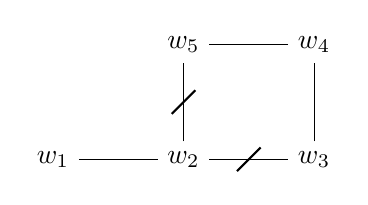
\begin{tikzpicture}[>=stealth']
{[start chain]
\node[on chain] (A) {$w_1$};
\node[on chain,join=by {-},right=of A] (B) {$w_2$};
\node[on chain,join=by {-},right=of B] (C) {$w_3$};
\node[on chain,join=by {-},above=of C] (D) {$w_4$};
\node[on chain,join=by {-},above=of B] (E) {$w_5$};}
\draw[-] (B) -- (E);
\coordinate (MidWay) at ($(B.east)!0.5!(C.west)$);
\draw [thick,-] ($(MidWay)-(\StrikeThru)$) -- ($(MidWay)+(\StrikeThru)$);
\coordinate (MidWay2) at ($(B.east)!0.5!(E.west)$);
\draw [thick,-] ($(MidWay2)-(\StrikeThru)$) -- ($(MidWay2)+(\StrikeThru)$);
\end{tikzpicture}
\end{center}
\end{figure}

This is called an action ledger conflict. Even with an action ledger traceback being done it is possible for items or funds to be duplicated. To mitigate situations like this is should be common practice to avoid joining worlds that have player history that collides. Another possible combatant is \textbf{item ledgers} (\ref{IL}) and \textbf{exchanges rates} (\ref{ER}).

\end{document}
